\graphicspath{{images/}}
\section*{Kontextfreie Grammatiken}

\begin{definition}{Kontextfreie Grammatik}\\
    Eine KontextFreie Grammatik $G(K F G)$ ist ein 4-Tupel $(N, \Sigma, P, A)$ mit

    \begin{itemize}
    \item $\quad N$ ist das Alphabet der Nichtterminale (Variablen)
    \item $\quad \Sigma$ ist das Alphabet der Terminale
    \item $\quad P$ ist eine endliche Menge von Produktionen mit der Form $X \rightarrow \beta$
    \end{itemize}

    Mit Kopf $X \in N$ und Rumpf $\beta \in(N \cup \Sigma)^{*}$

    \begin{itemize}
    \item $A$ ist das Startsymbol, wobei $A \in N$
    \end{itemize}

    Ein Wort $\beta \in(N \cup \Sigma)^{*}$ nennen wir Satzform.

    Seien $\alpha, \beta$ und $\gamma$ Satzformen und $A \rightarrow \gamma$ eine Produktion.

    \begin{itemize}
    \item Ableitungsschritt mit Produktion $A \rightarrow \gamma \quad \alpha A \beta \rightarrow \alpha \gamma \beta$
    \item Ableitung Folge von Ableitungsschritten $\alpha \rightarrow \cdots \rightarrow \omega$
    \end{itemize}
\end{definition}

\begin{definition}{Ableitungsbaum}\\
    Eine Ableitung kann als Ableitungsbaum / Parsebaum dargestellt werden. KGF $G_{1}$ für die Sprache $\left\{0^{n} 1^{m} \mid n, m \in N\right\}$

    \begin{itemize}
    \item $G_{1}=\{\{A, B, C\},\{0,1\}, P, A\}$
    \item $P=\{A \rightarrow B C, B \rightarrow 0 B|0| \varepsilon, C \rightarrow 1 C|1| \varepsilon\}$
    \end{itemize}

    Ableitung von $\omega_{1}=011$

    \begin{itemize}
    \item $A \rightarrow B C \rightarrow 0 A A \rightarrow 01 C \rightarrow 011 \rightarrow \ldots \rightarrow 011$
    \end{itemize}
    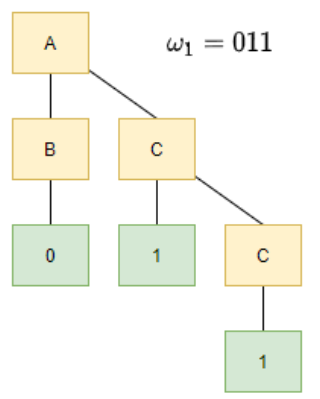
\includegraphics[width=0.3\linewidth]{ableitungsbaum.png}
\end{definition}

\begin{concept}{Mehrdeutigkeit}\\
    Eine KFG nennen wir mehrdeutig, wenn es ein Wort gibt, das mehrere Ableitungsbäume besitzt.\\
    \textbf{Mehrdeutigkeiten eliminieren:}
    \begin{itemize}
    \item Korrekte Klammerung vom Benutzer erzwingen
    \item Grammatik anpassen
    \item Den Produktionen einen Vorrang vergeben
    \end{itemize}
\end{concept}

\begin{KR}{KFG für Sprache L}\\
    Jede reguläre Sprache kann durch eine kontextfreie Grammatik beschrieben werden. Sei $L$ eine reguläre Sprache. Dann gibt es einen DEA $M=\left(Q, \Sigma, \delta, q_{0}, F\right)$ mit $L(M)=L$\\
    Dann können wir einen KFG für $L$ wie folgt bauen:
    \begin{itemize}
    \item Für jeden Zustand $q_{i}$ gibt es ein Nichtterminal $Q_{i}$
    \item Für jede Transition $\delta\left(q_{i}, a\right)=q_{j}$ erstellen wir die Produktion $Q_{i} \rightarrow a Q_{j}$
    \item Für jeden akzeptierenden Zustand $q_{i} \in F$ erstellen wir die Produktion $Q_{i} \rightarrow \varepsilon$
    \item Das Nichtterminal $Q_{0}$ wird zum Startsymbol $A$.
    \end{itemize}
\end{KR}